\chapter{Laboratorio 1}
\section{Introduzione}
Il primo circuito realizzato in laboratorio è l'\textit{emmitter follower}, di cui si riporta lo schema:
\begin{figure}[h!]
	\centering
	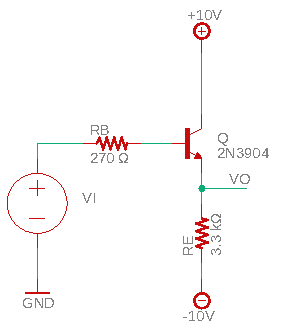
\includegraphics[width=0.4\linewidth]{./OtherFiles/Laboratorio 1/emitter follower}
	\caption{Schema del circuito emitter follower.}
	\label{fig:emitterfollwer}
\end{figure}

\noindent
Come si analizzerà in seguito, questo circuito presenta un guadagno unitario e può essere utilizzato per disaccoppiare un circuito collegato in ingresso da quello collegato in uscita.

\section{Emitter follower: punto di lavoro}
Per analizzare il circuito, si procede con l'analisi del punto di lavoro, dove i generatori di tensioni e correnti alternate vengono sostituiti rispettivamente da un corto circuito e da un circuito aperto (\Fig\ref{fig:emitterfollwer_puntodilavoro}).
\begin{figure}[h!]
	\centering
	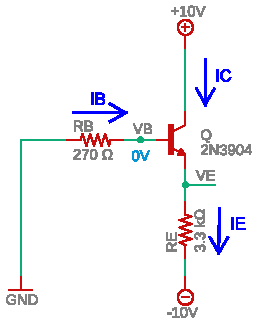
\includegraphics[width=0.4\linewidth]{./OtherFiles/Laboratorio 1/emitter follower_punto di lavoro_printout}
	\caption{Analisi del punto di lavoro del circuito emitter follower.}
	\label{fig:emitterfollwer_puntodilavoro}
\end{figure}
In particolare, il generatore di tensione (di segnale) v\textsubscript{i} viene quindi considerato come un corto circuito che collega un terminale della resistenza R\textsubscript{B} a massa. Considerando il modello ideale del transistor Q, con $\beta\overrightarrow{}\infty$ e corrente di base I\sub{B} nulla, si ricava che la corrente che attraversa la resistenza R\textsubscript{B} è nulla. Per cui, per la legge di Ohm $V=RI$, la caduta di potenziale sulla resistenza è nulla. Quindi il nodo V\textsubscript{B} si trova a una tensione di \SI{0}{\volt}. Se si esegue un bilancio di correnti sul nodo del transistor si ottiene $I\sub{B}+I\sub{C}=I\sub{E}$. Dal momento che la corrente I\sub{B} è nulla, I\sub{C} = I\sub{E}. La corrente di emettitore (e di conseguenza anche la corrente di collettore) si ricava dalla legge di Ohm: $I_E=I_C=\frac{\Delta V}{R_E}=\frac{V_O-(-\SI{10}{\volt})}{R_E}$. Infine, supponendo che il transistor si trovi in regione attiva diretta, $V_{BE}=V_{BO}=+\SI{0.7}{\volt}$. Quindi, $V_O=V_B-\SI{0.7}{\volt}= -\SI{0.7}{\volt}$. Si verifica l'ipotesi che il transistor si trova in regione attiva diretta, dal momento che $V_{CB}>0$. Avendo ricavato la corrente di collettore stazionaria, è utile calcolare anche la transconduttanza del transistor $g_m=\frac{I_C}{\phi_T}$, con $I_C$ corrente di collettore stazionaria e $\phi_T\simeq\SI{26}{\milli\volt}$. Essa sarà utile nell'analisi di piccolo segnale.

Nella seguente tabella, si riportano i valori teorici delle diverse grandezze che determinano il punto di lavoro, ottenute sostituendo i valori dei componenti utilizzati nel circuito. Questi valori dovranno essere confrontati con quelli misurati sul circuito reale.

\begin{table}[h!]
	\centering
	\begin{tabular}{c|c|c|c|c|c}
		\hline
		V\sub{B} [V] & V\sub{O} [V] & I\sub{B} [A] & I\sub{E} [mA] & I\sub{C} [mA] & g\sub{m} [A/V]\\ \hline
		0 & -0.7 & 0 & 2.818 & 2.818 & 0.1084\\ \hline
	\end{tabular}
\end{table}

\section{Emitter follower: analisi per piccolo segnale}
Consideriamo ora l'analisi per piccolo segnale del circuito. Il transistor viene sostituito con il suo modello per piccoli segnali a bassa frequenza senza resistenza di base e si procede spegnendo i generatori di grandezze continue, ottenendo il circuito mostrato in figura \ref{fig:emitterfollwer_piccolo segnale}. Come si può notare, il transistor è sostituito da un generatore di corrente ideale controllato dalla tensione $v_{be}$ e il terminale di base rimane isolato rispetto al collettore e all'emettitore. La transconduttanza \textit{g\sub{m}} è quella calcolata nell'analisi DC.
\begin{figure}[h!]
	\centering
	\includegraphics[width=0.4\linewidth]{./OtherFiles/Laboratorio 1/emitter follower\_piccolo segnale\_printout}
	\caption{Analisi di piccolo segnale del circuito emitter follower.}
	\label{fig:emitterfollwer_piccolo segnale}
\end{figure}
Si noti che la tensione v\sub{b} è pari a v\sub{i}, poiché la corrente nella resistenza R\sub{B} è nulla.
Per calcolare la funzione di trasferimento tra la tensione in ingresso v\sub{i} e la tensione in uscita v\sub{o}, si calcola il bilancio di correnti al nodo \textbf{E}:
\begin{equation}
	\begin{split}
		i_c&=g_mv_{be} = i_e \\ 
		v_b&=v_i \\
		v_e&=v_o \\
		i_c&=g_m(v_b-v_e)=g_m(v_i-v_o) \\
		i_e&=\frac{v_e-\SI{0}{\volt}}{R_E}=\frac{v_o}{R_E} \\
		\frac{v_o}{R_E}&=g_m(v_i-v_o) \\
		\frac{v_o}{v_i}&=\frac{g_m R_E}{1+g_m R_E}\simeq 1 \; per \; g_m R_E\gg 1 .\\
	\end{split}
\end{equation}
Si realizza quindi un circuito a guadagno unitario.

\section{Componenti e misure}
Il circuito è stato realizzato in laboratorio su una breadboard e il risultato è visibile in figura \ref{fig:emitterfollwer_circuito}. Inizialmente, non è stato collegato il generatore di forme d'onda v\sub{i} in ingresso al circuito, sostituendolo con un collegamento a massa. In questo modo è possibile effettuare l'analisi del punto di lavoro del circuito.
\begin{figure}[h!]
	\centering
	\includegraphics[width=0.6\linewidth]{./ImageFiles/Laboratorio 1/IMG\_20220510\_103526}
	\caption{Foto del circuito realizzato in laboratorio.}
	\label{fig:emitterfollwer_circuito}
\end{figure}

\noindent
Per realizzare il circuito sono stati utilizzati i seguenti componenti: 
\begin{itemize}
	\item transistor 2N3904;
	\item una resistenza da \SI{270}{\ohm} per realizzare la resistenza R\sub{B};
	\item due resistenze rispettivamente da R\sub{E1}=\SI{1.5}{\ohm} e R\sub{E2}=\SI{1.8}{\ohm} connesse in parallelo per realizzare la resistenza R\sub{E}.
\end{itemize}
Inoltre, sono stati utilizzati i seguenti strumenti:
\begin{itemize}
	\item alimentatore da banco con tensione positiva \SI{10}{\volt}, tensione negativa \SI{-10}{\volt} e limite in corrente di \SI{50}{\milli\ampere};
	\item oscilloscopio a due canali;
	\item generatore di forme d'onda;
	\item multimetro da banco.
\end{itemize}

\noindent
Prima di realizzare il circuito, si sono misurati attraverso il multimetro i valori delle resistenze utilizzate e delle tensioni delle giunzioni P-N tra \textit{base} e \textit{collettore} e tra \textit{base} e \textit{emettitore} del transistor, ottenendo le seguenti misure:

\begin{table}[h!]
	\centering
	\begin{tabular}{c|c|c}
		\hline
		Componente & Valore nominale & Valore misurato \\ \hline
		R\sub{B} & \SI{270}{\ohm} & \SI{279}{\ohm}  \\ \hline
		R\sub{E1} &\SI{1.5}{\kilo\ohm} & \SI{1.495}{\kilo\ohm} \\ \hline
		R\sub{E2} &\SI{1.8}{\kilo\ohm} & \SI{1.810}{\kilo\ohm} \\ \hline
		Vd\sub{B-E} & $\simeq$ \SI{0.7}{\volt} & \SI{0.700}{\volt} \\ \hline
		Vd\sub{B-C} & $\simeq$ \SI{0.7}{\volt} & \SI{0.679}{\volt} \\ \hline
	\end{tabular}
\end{table}

\noindent
Si noti che le tensioni delle giunzioni P-N hanno valori diversi: ciò è dovuto alla tecnologia di realizzazione del transistor (tecnologia planare), nella quale le due giunzioni hanno una diversa lunghezza.

Una volta realizzato il circuito, sono state misurate le tensioni ai nodi V\sub{B} e V\sub{O} da cui è possibile ricavare (tramite la legge di Ohm) le correnti di base e di emettitore. La corrente di collettore si ricava come differenza tra la corrente di emettitore e corrente di base. Inoltre, è possibile calcolare la transconduttanza come rapporto tra la corrente di collettore stazionaria e la tensione termica. 

\noindent
Sono stati ottenuti i seguenti valori:
\begin{table}[h!]
	\centering
	\begin{tabular}{c|c|c|c|c|c}
		\hline
		V\sub{B} [mV] & V\sub{O} [V] & I\sub{B} [mA] & I\sub{E} [mA] & I\sub{C} [mA] & g\sub{m} [A/V]\\ \hline
		-3.820 & -0.655 & 0.014 & 2.819 & 2.805 & 0.1079\\ \hline
	\end{tabular}
\end{table}

\noindent
I valori misurati sono molto simili ai valori calcolati nell'analisi teorica del punto stazionario. In particolare, si noti che la corrente di base, pur non essendo nulla, assume un valore molto piccolo (\SI{14}{\micro\ampere}).

Successivamente, si è applicato un segnale sinusoidale v\sub{i} tramite un cavo di tipo BNC collegato al generatore di forme d'onda, impostando una frequenza pari a \textit{f=}\SI{1}{\kilo\hertz} e una tensione picco-picco \textit{V\sub{pp}=}\SI{2}{\volt}. Collegando opportunamente i connettori dell'oscilloscopio, è stato possibile misurare il segnale in ingresso e in uscita al circuito. \`E stato possibile verificare che il guadagno del cicrcuito è effettivamente unitario (\Fig\ref{fig:emitterfollwer_oscilloscopio_1}).
\begin{figure}[t]
	\centering
	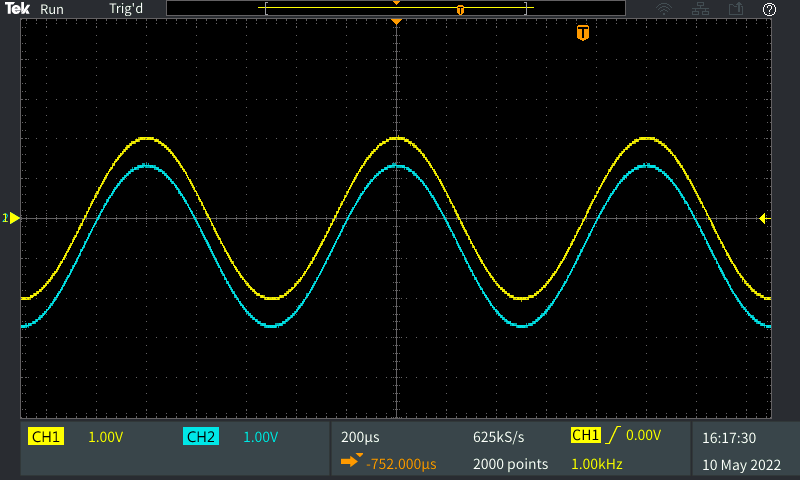
\includegraphics[width=0.7\linewidth]{./ImageFiles/Laboratorio 1/TEK00005}
	\caption{Segnale in ingresso (CH1) e in uscita (CH2) all'emitter follower misurato con l'oscilloscopio. L'onda sinusoidale in ingresso ha frequenza \SI{1}{\kilo\hertz} e tensione picco-picco di \SI{2}{\volt}.}
	\label{fig:emitterfollwer_oscilloscopio_1}
\end{figure}
Si noti come il segnale giallo (ingresso) e il segnale azzurro (uscita) abbiano uguale ampiezza e fase. Per verificare lo sfasamento, è possibile selezionare la modalità XY sull'oscilloscopio e analizzare il grafico mostrato (\Fig\ref{fig:emitterfollwer_XY_1}).
\begin{figure}[h!]
	\centering
	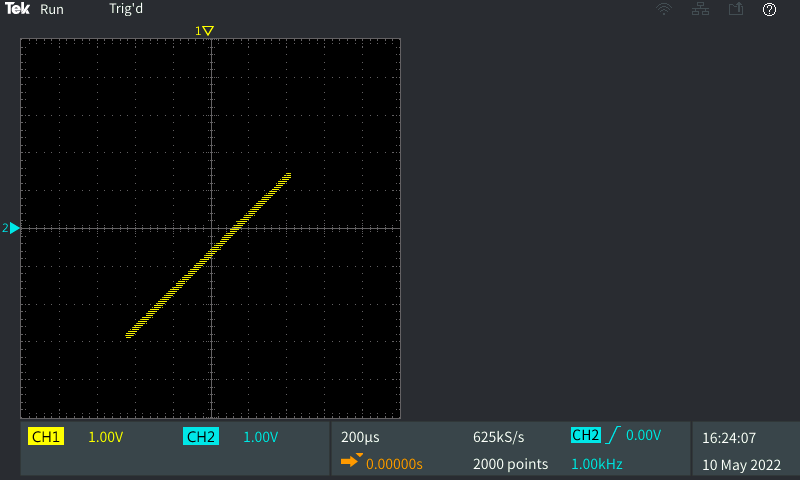
\includegraphics[width=0.7\linewidth]{./ImageFiles/Laboratorio 1/TEK00008}
	\caption{Grafico XY con onda sinusoidale in ingresso di frequenza \SI{1}{\kilo\hertz} e tensione picco-picco di \SI{2}{\volt}.}
	\label{fig:emitterfollwer_XY_1}
\end{figure}

\noindent
Come si può notare, la presenza di un segmento con inclinazione di 45 gradi indica che i segnali sono in fase. Inoltre, si noti che l'intersezione del segmento con l'asse delle ordinate rappresenta l'offset, di circa \SI{0.7}{\volt}, dovuto alla giunzione base-emettitore. 
Tuttavia, aumentando la frequenza dell'onda sinusoidale fino ai \SI{10}{\mega\hertz}, il circuito introduce uno sfasamento. Infatti, a frequenze elevate le non idealità del transistor diventano significative. Per questo motivo, il grafico XY (\Fig\ref{fig:emitterfollwer_XY_2}) non mostra più un segmento ma un ellissi, che indica la presenza di uno sfasamento. 
\begin{figure}[h!]
	\centering
	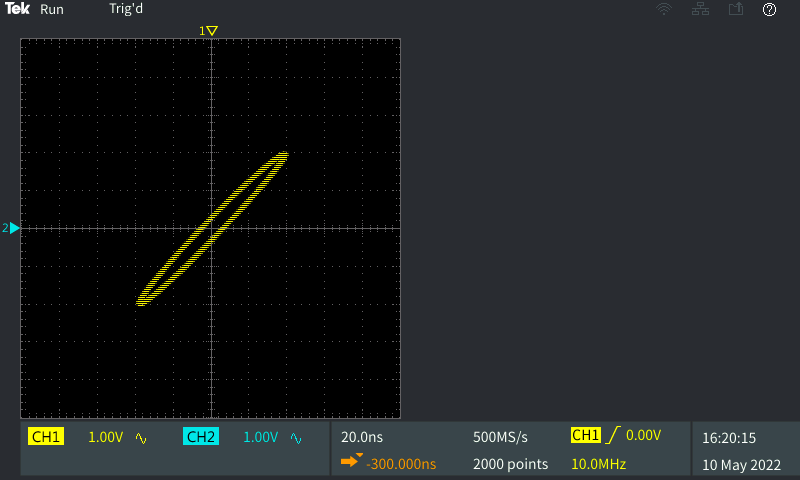
\includegraphics[width=0.7\linewidth]{./ImageFiles/Laboratorio 1/TEK00006}
	\caption{Grafico XY con onda sinusoidale in ingresso con frequenza \SI{10}{\mega\hertz} e tensione picco-picco di \SI{2}{\volt}. I segnali in ingresso sono stati accoppiati in AC.}
	\label{fig:emitterfollwer_XY_2}
\end{figure}
La differenza di fase tra i segnali è visibile anche utilizzando la rappresentazione sull'asse dei tempi come mostrato in figura \ref{fig:emitterfollwer_oscilloscopio_2}.
\begin{figure}[h!]
	\centering
	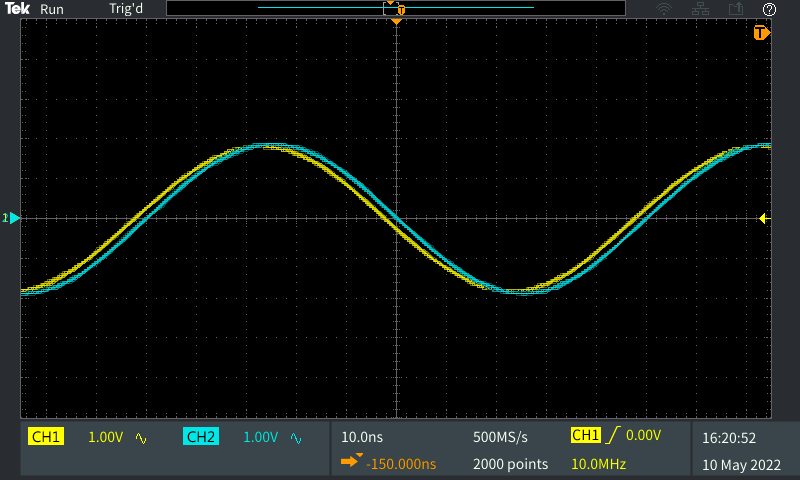
\includegraphics[width=0.7\linewidth]{./ImageFiles/Laboratorio 1/TEK00007}
	\caption{Segnale in ingresso (CH1) e in uscita (CH2) all'emitter follower misurato con l'oscilloscopio. L'onda sinusoidale in ingresso ha frequenza \SI{10}{\mega\hertz} e tensione picco-picco di \SI{2}{\volt}. I segnali in ingresso sono stati accoppiati in AC.}
	\label{fig:emitterfollwer_oscilloscopio_2}
\end{figure}

\noindent
Osservando i grafici delle tensioni ingresso-uscita è possibile notare che il circuito ha guadagno unitario. Tuttavia, un'analisi più approfondita sul guadagno del circuito è stata svolta nella attività di laboratorio successiva.